\chapter{Accesso selettivo e privato ai Data center Outsourced}

\section{Introduzione}
La crescente quantità di informazioni generate, raccolte, condivise e diffuse al giorno d'oggi rende sempre più difficile ed economicamente costosa la gestione interna dei data center da parte di aziende private e pubbliche. L'ampia disponibilità di fornitori di cloud che offrono servizi di alta qualità per l'archiviazione e la gestione dei dati è quindi una motivazione che spinge le aziende a spostare sempre più spesso i propri data center nel cloud. Sebbene questa tendenza presenti chiari vantaggi economici, introduce anche nuovi problemi di sicurezza. Infatti, quando si sposta un data center nel cloud, i dati non sono più sotto il controllo diretto del proprietario che deve affidarsi a un sistema esterno per fornire le stesse garanzie della gestione interna (ad esempio, disponibilità dei dati, protezione da attacchi esterni, accesso selettivo ai dati, gestione della tolleranza ai guasti). Tuttavia, essendo terze parti esterne, si presume spesso che i fornitori di cloud siano onesti ma curiosi, quindi affidabili nel gestire correttamente i dati che memorizzano, ma non nell'accedere ai loro contenuti. Questa situazione solleva diverse preoccupazioni, soprattutto per quanto riguarda l'adeguata protezione della riservatezza dei dati. Una soluzione efficace consiste nel crittografare i dati prima di esternalizzarli, in modo che le parti non autorizzate (compreso il cloud provider), non conoscendo la chiave di crittografia, non possano accedere al contenuto dei dati in chiaro. La crittografia dei dati prima dell'outsourcing presenta tuttavia alcuni svantaggi.
\\
\newline
In primo luogo, pur nascondendo efficacemente i dati in chiaro agli occhi del fornitore, la crittografia di tutti i dati con un'unica chiave richiederebbe che tutti gli utenti abbiano una visibilità completa delle risorse della raccolta dati, oppure che il data owner medi le richieste di accesso ai dati per imporre un accesso selettivo. In secondo luogo, la crittografia complica la valutazione delle query, poiché il cloud provider non può valutare direttamente le query degli utenti sui dati crittografati. In terzo luogo, nei casi in cui anche le query poste dagli utenti devono essere protette, la crittografia potrebbe non fornire sufficienti garanzie di protezione. Per superare questi problemi, sono state proposte diverse tecniche che mirano a supportare un accesso selettivo e privato ai dati esternalizzati. Queste tecniche si basano sull'uso di una crittografia selettiva, nel senso che i diversi pezzi di dati vengono crittografati con chiavi diverse a seconda di chi può accedervi. Gli indici sono invece utilizzati dai cloud provider per selezionare i dati da restituire in risposta a una query, eventualmente anche senza rivelare l'obiettivo della query stessa. Sebbene, singolarmente, queste tecniche rappresentino soluzioni efficaci, l'adozione combinata di crittografia selettiva e indici può causare violazioni della riservatezza che devono essere affrontate con attenzione.
\\
\newline
In questo capitolo presentiamo una panoramica delle tecniche proposte per consentire ai dati di auto-applicare la politica di controllo degli accessi definita dal loro proprietario e per supportare la valutazione delle query sui dati criptati. La Figura 1 illustra lo scenario di riferimento in cui il data owner affida i propri dati a un fornitore di cloud e gli utenti accedono a tali dati.
Il resto del capitolo è organizzato come segue: 
\begin{itemize}
    \item La sezione 2 mostra come i dati criptati possano imporre restrizioni al controllo degli accessi, senza richiedere l'intervento del data owner o la collaborazione del server di archiviazione.
    \item La sezione 3 presenta una panoramica delle tecniche proposte per supportare la valutazione delle query su dati criptati.
    \item La sezione 4 descrive nuove soluzioni per accedere a raccolte di dati in outsourcing senza rivelare al server di archiviazione l'obiettivo dell'interrogazione.
    \item La sezione 5 illustra i problemi di privacy che sorgono quando si combinano soluzioni per l'applicazione del controllo degli accessi con tecniche di indicizzazione e introduce soluzioni preliminari a questo problema.
    \item La Sezione 6 presenta le nostre osservazioni conclusive.
\end{itemize}

\begin{figure}[h]
    \centering
    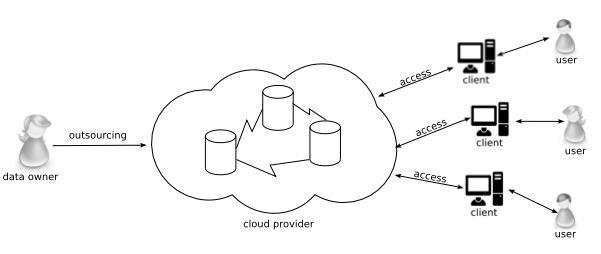
\includegraphics[width=1\linewidth]{paper_selective-and-private-access-to-outsourced-data-centers/image0.png}
    \label{fig-1}
\end{figure}

\section{Access Control Enforcement}
Le informazioni memorizzate nei data center possono essere di qualsiasi tipo: database relazionali, documenti XML, file multimediali, ecc. Per semplicità, ma senza perdita di generalità, in questo capitolo assumiamo che i dati memorizzati nel cloud siano organizzati in un database relazionale, con la nota che tutti gli approcci illustrati nel seguito possono essere facilmente adattati per operare su qualsiasi modellazione logica dei dati.
\\
\newline
Quindi consideriamo una relazione $r$ definita sullo schema $R(a_1,...,a_n)$, dove l'attributo $a_i$ è definito sul dominio $D_i, i = 1,...,n$. 
Al server che ha i dati, la relazione $r$ è rappresentata come una relazione $r^k$, definita sullo schema $R^k(tid,enc)$, con $tid$ la chiave primaria numerica aggiunta alla relazione crittata e $enc$ la tupla crittata.
\\
Ogni tupla $t$ in $r$ è rappresentata come una tupla crittata $t^k$ in $r^k$, dove $t^k[tid]$ è scelto randomicamente dal data owner, e $t^k[enc]=E_k(t)$, con $E$ una funzione di crittazione simmetrica con chiave $k$
\\
\newline
Sono state proposte diverse tecniche per applicare il controllo degli accessi senza l'intervento né del server di archiviazione, per motivi di riservatezza, né del data owner, per motivi di efficienza.
Queste soluzioni si basano sull'idea che i dati si \textit{auto-applichino(self-enforce)} alle restrizioni di accesso selettivo attraverso la crittografia, come illustrato nel seguito di questa sezione.

\subsection{Selective Encryption}
Una soluzione promettente per imporre il controllo degli accessi ai dati in outsourcing si basa sulla crittografia selettiva, che adotta chiavi di crittografia diverse per tuple diverse e distribuisce selettivamente le chiavi agli utenti autorizzati. Ogni utente può decifrare e quindi accedere a un sottoinsieme di tuple, a seconda delle chiavi che conosce. La politica di autorizzazione che regola quale utente può leggere quale tupla è definita dal data owner prima di esternalizzare la relazione $r$
\\
\newline
La politica di autorizzazione può essere rappresentata come una matrice binaria di accesso $M$ con una riga per ogni utente $u$ e una colonna per ogni tupla $t$, dove:\\
\newline
$\begin{cases}
    M[u,t]=1 \text{ se u può accedere a t};\\
    M[u,t]=0 \text{ altrimenti}.   
\end{cases}$\\
\newline
per illustrare, considera la relazione PATIENTS nella tabella sottostante:

\begin{figure}[h!]
    \centering
    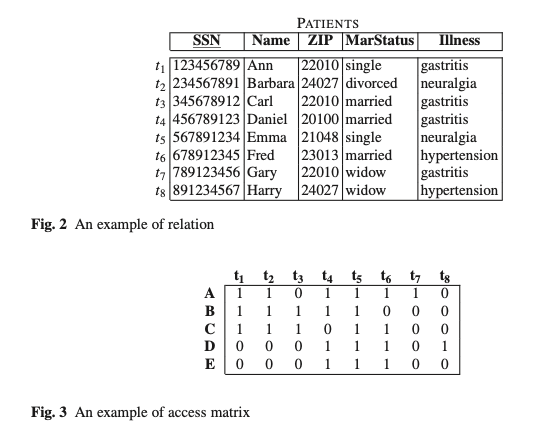
\includegraphics[width=1\linewidth]{paper_selective-and-private-access-to-outsourced-data-centers/image1.png}
    \label{fig:fig-2}
\end{figure}
$\\$
La Figura 3 illustra un esempio di matrice di accesso che regola l'accesso alle tuple della relazione PATIENTS da parte degli utenti A, B, C, D ed E. La $j_{esima}$ colonna della matrice rappresenta la lista di controllo degli accessi $acl(t_j)$ della tupla $t_j$, per ogni $j= 1,..., |r|.$ Ad esempio, con riferimento alla matrice di Figura 3, $acl(t_1)=ABC$.\\
La politica di cifratura, che definisce e regola l'insieme delle chiavi utilizzate per cifrare le tuple e la distribuzione delle chiavi agli utenti, deve essere equivalente alla politica di autorizzazione, nel senso che ogni utente deve poter decifrare tutte e solo le tuple a cui è autorizzato ad accedere.
Le soluzioni che traducono una politica di autorizzazione in una politica di crittografia equivalente hanno due principali desiderata progettuali: 
\begin{enumerate}[label=\roman*)]
    \item garantire che ogni utente debba gestire una sola chiave;
    \item crittografare ogni tupla con una sola chiave (cioè, nessuna tupla viene replicata).
\end{enumerate}
Per soddisfare questi due requisiti, gli approcci di crittografia selettiva si basano su tecniche di derivazione delle chiavi che permettono di calcolare una chiave di crittografia $k_j$ a partire dalla conoscenza di un'altra chiave $k_i$ e (eventualmente) di un'informazione disponibile al pubblico.\\
Per determinare quale chiave può essere derivata da quale altra chiave, le tecniche di derivazione delle chiavi richiedono la definizione preliminare di \textit{key derivation hierarchy}. Una gerarchia di derivazione delle chiavi può essere rappresentata graficamente come un grafo diretto con un vertice $v_i$ per ogni chiave $k_i$ del sistema e un arco $(v_i,v_j)$ dalla chiave $k_i$ alla chiave $k_j$ $sse$ $k_j$ può essere derivata direttamente da $k_i$.\\
\newline
Si noti che la derivazione delle chiavi può essere applicata a catena, nel senso che la chiave $k_j$ può essere calcolata a partire dalla chiave $k_i$ se esiste un percorso (di lunghezza arbitraria) da $v_i$ a $v_j$ nella gerarchia di derivazione delle chiavi.
Una gerarchia di derivazione delle chiavi può avere forme diverse, come descritto di seguito.
\begin{itemize}
    \item \textit{Chain of vertices}: la chiave $k_i$ associata al vertice $v_j$ è calcolata applicando la funzione \textit{one-way} alla chiave $k_i$ del predecessore nella catena. Nessuna informazione pubblica è necessaria
    \item \textit{Tree hierarchy}: la chiave $k_i$ associata al vertice $v_j$ è calcolata applicando la funzione \textit{one-way} alla chiave $k_i$ del suo antenato diretto, e una label pubblica $l_j$ associata con $k_j$. Le label pubbliche sono necessarie per garantire che i diversi figli di uno stesso nodo dell'albero abbiano chiavi diverse.
    \item \textit{DAG hierarchy}: le chiavi nella gerarchia possono avere più di un antenato diretto e ogni arco della gerarchia è associato a un token pubblicamente disponibile. Date due chiavi $k_i$ e $k_j$ , e l'etichetta pubblica $l_j$ di $k_j$ , il token $t_{i,j}$ permette di calcolare $k_j$ a partire da $k_i$ e $l_j$ . Il token $t_{i,j}$ è calcolato come $t_{i,j}=k_j$ $\oplus$ $(k_i,l_j)$, dove $\oplus$ è l'operatore XOR bitwise e $f$ è una funzione crittografica deterministica. Tramite $t_{i,j}$, tutti gli utenti che conoscono (o sono in grado di ricavare) la chiave $k_i$ possono ricavare anche la chiave $k_j$
\end{itemize}

\section{BEL e SEL}
In caso di modifiche alla politica di autorizzazione, la politica di crittografia deve essere aggiornata di conseguenza, per garantire la loro equivalenza. Poiché la chiave utilizzata per criptare ogni tupla $t$ in $r$ dipende dall'insieme di utenti che possono accedervi, potrebbe essere necessario criptare nuovamente le tuple coinvolte nell'aggiornamento della politica con una chiave diversa che solo gli utenti delle nuove liste di controllo degli accessi conoscono o possono ricavare. Un approccio banale per imporre un'operazione di grant/revoke sulla tupla $t$ richiede che il data owner:
\begin{enumerate}[label=\roman*)]
    \item scarichi $t_k$ dal server;
    \item la decifri;
    \item aggiorni la gerarchia di derivazione delle chiavi se non include un vertice che rappresenta il nuovo insieme di utenti in $acl(t)$;
    \item cripti $t$ con la chiave $k'$ associata al vertice che rappresenta $acl(t)$;
    \item eventualmente aggiorni il catalogo pubblico contenente i token.
\end{enumerate}
Ad esempio, si consideri la politica di crittografia delle figura sottostante:
\begin{figure}[h!]
    \centering
    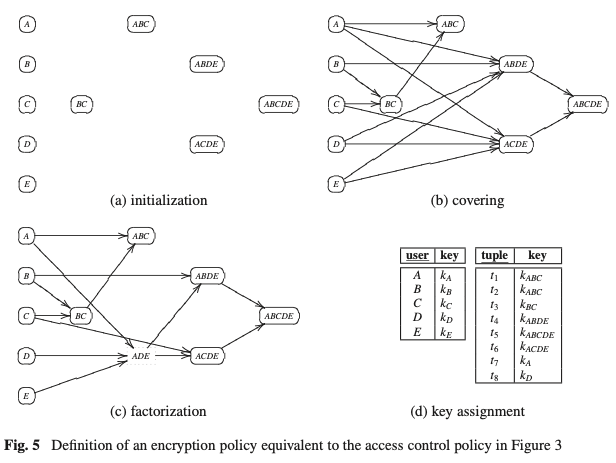
\includegraphics[width=1\linewidth]{paper_selective-and-private-access-to-outsourced-data-centers/image2.png}
    \label{fig:fig-3}
\end{figure}
\\
e si supponga che all'utente $D$ sia concesso l'accesso alla tupla $t_1$. Il data owner dovrebbe scaricare $t^k_1$; decifrarla usando la chiave $k_{ABC}$; inserire un vertice che rappresenti $acl(t_1)=ABCD$ nella gerarchia di derivazione delle chiavi; criptare $t_1$ con $k_{ABCD}$; e caricare la tupla criptata sul server, insieme ai token necessari agli utenti A, B, C e D per derivare $k_{ABCD}$. Questo approccio, pur essendo efficace e in grado di imporre correttamente gli aggiornamenti dell'autorizzazione, lascia al data owner l'onere di gestire l'aggiornamento. Inoltre, le operazioni di ricrittografia sono computazionalmente costose. Per limitare l'overhead del data owner, gli autori propongono di utilizzare due livelli di crittografia (ciascuno caratterizzato da una propria politica di crittografia) per delegare parzialmente al server la gestione delle operazioni di grant e revoke.
\begin{itemize}
    \item Il \textit{Base Encryption Level(BEL)} viene applicato dal data owner prima di esternalizzare il set di dati. La gerarchia di derivazione delle chiavi BEL viene costruita in base alla politica di autorizzazione esistente al momento dell'inizializzazione. In caso di aggiornamento della politica, la BEL viene aggiornata solo inserendo eventualmente dei token nel catalogo pubblico (ovvero dei bordi nella gerarchia di derivazione delle chiavi BEL).\\
    Si noti che ogni vertice $v$ nella gerarchia di derivazione delle chiavi BEL ha due chiavi: una chiave di derivazione $k$ (utilizzata solo per la derivazione delle chiavi) e una chiave di accesso $k_a$ (utilizzata per crittografare le tuple, ma che non può essere sfruttata ai fini della derivazione delle chiavi).
    \item Il \textit{Il Surface Encryption Layer(SEL)}viene applicato dal server sulle tuple che sono già state crittografate dal data owner a BEL. Il server applica dinamicamente gli aggiornamenti dei criteri di autorizzazione, eventualmente cifrando nuovamente le tuple e modificando la gerarchia di derivazione delle chiavi del SEL per riflettere correttamente gli aggiornamenti. A differenza di BEL, i vertici della gerarchia di derivazione delle chiavi di SEL sono associati a una singola chiave $k_s$
\end{itemize}
Intuitivamente, con l'approccio di over-encryption, un utente può accedere a una tupla $t$ solo se conosce le chiavi utilizzate per crittografare $t$ in BEL e SEL. Al momento dell'inizializzazione, le politiche di crittografia di BEL e SEL coincidono, ma cambiano immediatamente e diventano diverse a ogni aggiornamento della politica. Le operazioni di grant e revoke sono applicate come segue:
\begin{itemize}
    \item \textit{Grant}: Quando l'utente $u$ ottiene l'accesso alla tupla $t$, deve conoscere la chiave utilizzata per crittografare $t$ sia in BEL che in SEL. Pertanto, il proprietario dei dati aggiunge un token nella gerarchia di derivazione delle chiavi di BEL dal vertice che rappresenta $u$ al vertice la cui chiave è stata utilizzata per crittografare $t$ (cioè il vertice che rappresenta $acl(t)$ al momento dell'inizializzazione).
    Il proprietario chiede quindi al server di aggiornare la gerarchia di derivazione delle chiavi in SEL ed eventualmente di criptare nuovamente le tuple. La tupla $t$ deve infatti essere cifrata al SEL con la chiave del vertice che rappresenta $acl(t) \cup \{u\}$ (che viene eventualmente inserito nella gerarchia). Oltre a $t$, anche altre tuple possono aver bisogno di essere ricifrate al SEL per garantire la corretta applicazione dell'aggiornamento della politica. Infatti, le tuple criptate con la stessa chiave di $t$ a BEL e che l'utente $u$ non può leggere devono essere criptate a SEL con una chiave che $u$ non conosce (e non può ricavare).
    Il proprietario dei dati deve quindi assicurarsi che ogni tupla $t_i$ che condivide la chiave di cifratura BEL con $t$ sia cifrata in SEL con la chiave del vertice che rappresenta $acl(t_i)$. Ad esempio, si consideri la matrice di accesso della Figura 3 e le politiche di crittografia di BEL e SEL che la applicano.
    BEL e SEL che la applicano nella Figura 6, e supponiamo che all'utente $D$ sia concesso l'accesso alla tupla $t_1$. La Figura 7 illustra le politiche di crittografia di BEL e SEL dopo l'applicazione dell'operazione di grant.\\
    \newline
    Per applicare questa modifica alla politica di controllo degli accessi, il proprietario dei dati deve innanzitutto aggiungere un token che consenta all'utente $D$ di derivare la chiave di accesso del vertice $ABC(k^a_{ABC})$ utilizzata per crittografare $t_1$ a BEL (bordo tratteggiato nella figura). Inoltre, chiederà al server di aggiornare la gerarchia di derivazione delle chiavi SEL per aggiungere un vertice che rappresenti $ABCD$. La tupla $t_1$ viene quindi sovracrittografata in SEL con la chiave di questo nuovo vertice.

    \item \textit{Revoke}: Quando l'utente $u$ perde il privilegio di accedere alla tupla $t$, il proprietario dei dati chiede semplicemente al server di criptare nuovamente (a SEL) la tupla con la chiave associata all'insieme $acl(t)\backslash\{u\}$ di utenti. Se il vertice che rappresenta questo insieme di utenti non è rappresentato nella gerarchia di derivazione delle chiavi di SEL, il server aggiorna prima la gerarchia inserendo il nuovo vertice e poi cripta nuovamente la tupla. Ad esempio, si considerino le politiche di cifratura di BEL e SEL nella Figura 7 e si supponga che il proprietario dei dati revochi a $B$ il privilegio di accedere a $t_4$. Il proprietario dei dati richiede al server di modificare SEL (BEL non è influenzato dalle operazioni di revoke) per garantire che la tupla $t_4$ sia crittografata con una chiave che l'utente $B$ non può ricavare. A tal fine, $t_4$ viene nuovamente crittografata con la chiave $k^s_{ADE}$ . La Figura 8 illustra le politiche di crittografia di BEL e SEL dopo l'applicazione dell'operazione di revoke. Si noti che il vertice $ABDE$ è stato rimosso dalla gerarchia poiché non è necessario per l'applicazione della politica né utile per ridurre il numero di token.
\end{itemize}

\begin{figure}[h!]
    \centering
    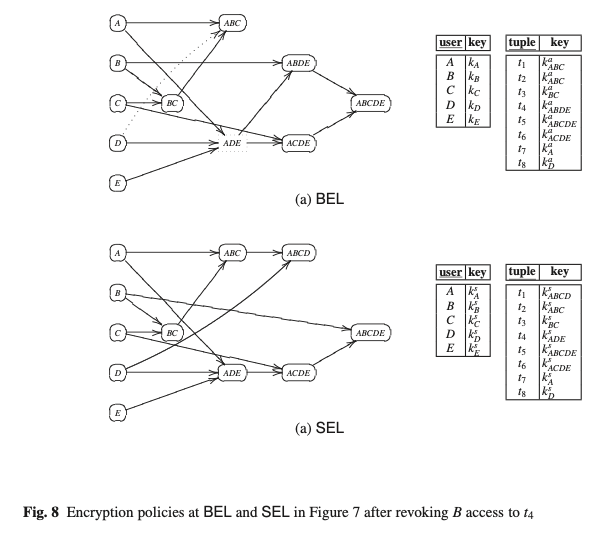
\includegraphics[width=1\linewidth]{paper_selective-and-private-access-to-outsourced-data-centers/image3.png}
\end{figure}
$\\$
Poiché la gestione delle operazioni di (ri)crittografia in SEL è delegata al server, esiste il rischio di collusioni con gli utenti. Infatti, combinando le loro conoscenze, un utente e il server possono decifrare tuple a cui né il server né l'utente possono accedere. Ad esempio, con riferimento alla politica di crittografia della Figura 8, il server e l'utente $D$ possono accedere alla tupla $t_2$ combinando le loro conoscenze. Infatti, questa tupla è cifrata con la chiave di accesso $k^a_{ABC}$ a BEL, nota all'utente $D$ in quanto utilizzata per cifrare $t_1$, e con la chiave $k^s_{ABC}$ a SEL, nota al server. La collusione rappresenta un rischio per la corretta applicazione della politica di autorizzazione, ma questo rischio è limitato. Infatti, la collusione tra un utente $u$ e il server permette di decifrare una tupla $t$ a cui non si è autorizzati ad accedere solo se a $u$ viene concesso il privilegio di leggere una tupla $t' \neq t$ (diversa da $t$) che è cifrata con la stessa chiave di $t$ a BEL. Infatti, $u$ conosce la chiave con cui $t$ è cifrato a BEL (in quanto necessaria per accedere a $t'$) mentre il server conosce la chiave con cui è cifrato a SEL (in quanto gestisce tutte le chiavi di cifratura a SEL).\\
Il rischio di collisione può quindi essere mitigato al prezzo di utilizzare un numero maggiore di chiavi a BEL, cioè utilizzando la stessa chiave di crittografia a BEL solo per le tuple le cui acl hanno la probabilità di evolvere nello stesso modo.

\subsection{Scrivere privilegi}
La soluzione descritta nella sezione precedente, pur imponendo efficacemente i privilegi di lettura e gli aggiornamenti, presuppone che la relazione in outsourcing sia di sola lettura (cioè che solo il proprietario possa modificare le tuple). Per consentire al proprietario dei dati di autorizzare selettivamente altri utenti ad aggiornare i dati esternalizzati, questo approccio è stato integrato con una tecnica specifica per gestire i privilegi di scrittura. L'approccio di [11] associa a ogni tupla un write tags (cioè un valore casuale indipendente dal contenuto della tupla) definito dal proprietario dei dati. L'accesso ai write tags è regolato attraverso una crittografia selettiva: il \textit{write tag} della tupla $t$ è crittografato con una chiave nota solo agli utenti autorizzati a scrivere $t$ (cioè gli utenti specificati nella sua lista di accesso alla scrittura, indicata con $acl_w(t)$) e dal server. In questo modo, solo il server e gli autori autorizzati hanno accesso al write tags in chiaro di ogni tupla. Il server accetterà quindi una richiesta di scrittura su una tupla quando l'utente richiedente dimostrerà di conoscere il write tags corrispondente.\\
\newline
Poiché la chiave utilizzata per crittografare il write tags di una tupla deve essere condivisa tra il server e gli autori di tuple, è necessario estendere la gerarchia di derivazione delle chiavi con il server di archiviazione. Tuttavia, il server non può accedere alle tuple esternalizzate in chiaro e quindi non può essere trattato come un ulteriore utente autorizzato (cioè con la possibilità di derivare le chiavi nella gerarchia). \\Le chiavi utilizzate per criptare i write tags sono quindi definite in modo tale che: 

\begin{enumerate}[label=\roman*)]
    \item gli utenti autorizzati possano calcolarle applicando una funzione di hash sicura a una chiave che già conoscono (o che possono ricavare tramite una sequenza di token);
    \item il server possa ricavarle direttamente da una chiave $k_S$ assegnatagli, tramite un token appositamente aggiunto alla gerarchia di derivazione delle chiavi.
\end{enumerate}
Si noti che le chiavi utilizzate per crittografare i write tags non possono essere utilizzate per derivare altre chiavi nella gerarchia. Ad esempio, si consideri la politica di crittografia delle figure 5(c-d) e si assuma che:\\
$acl_w(t_1)=acl_w(t_7)=A, acl_w(t_2)=acl_w(t_3)=BC, acl_w(t_4)=ADE, acl_w(t_5)=acl_w(t_8)=D e acl_w(t_6)=E$.\\
\newline
La Figura 9(a) illustra la gerarchia di derivazione delle chiavi, ampliata con la chiave kS assegnata al server S e le chiavi necessarie per crittografare i write tags (i vertici e gli spigoli aggiuntivi sono tratteggiati nella figura). Le figure 9(b-c) riassumono le chiavi assegnate agli utenti e al server e le chiavi utilizzate per crittografare le tuple della relazione PAZIENTI e i loro write tags, rispettivamente.

\begin{figure}[h!]
    \centering
    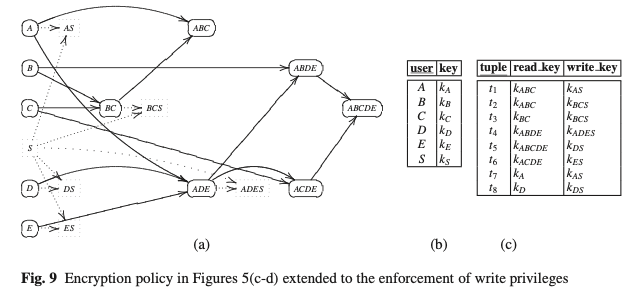
\includegraphics[width=1\linewidth]{paper_selective-and-private-access-to-outsourced-data-centers/image4.png}
\end{figure}

L'approccio dell'over-ecnryption, pur essendo efficace per imporre gli aggiornamenti di una politica di autorizzazione alla lettura, non può purtroppo essere adottato per imporre la concessione e la revoca delle autorizzazioni alla scrittura. Un possibile metodo per imporre privilegi di scrittura dinamici funziona come segue.

\begin{itemize}
    \item \textit{Grant}: Quando all'utente u viene concesso il privilegio di modificare la tupla $t$, il write tag viene crittografato con una chiave nota al server e agli utenti in $acl_w(t)\cup\{u\}$. Se la gerarchia di derivazione delle chiavi non la include, tale chiave viene creata e aggiunta correttamente alla gerarchia. Ad esempio, con riferimento alla politica di crittografia della Figura 9, si supponga che all'utente $B$ sia concesso il privilegio di scrittura su $t_4$. Il write tag della tupla deve essere crittografato con la chiave $k_{ABDES}$, che viene inserita nella gerarchia di derivazione delle chiavi, mentre la chiave $k_{ADES}$ può essere rimossa.
    \item \textit{Revoke}: Quando all'utente $u$ viene revocato il privilegio di scrittura sulla tupla $t$, è necessario definire un nuovo write tag per $t$, con un valore indipendente dal tag precedente (ad esempio, può essere scelto adottando una funzione casuale sicura). Questo è necessario per garantire che $u$, che non è ignaro, non possa sfruttare la sua conoscenza del precedente write tag della tupla $t$ per eseguire operazioni di scrittura non autorizzate. Dopo che il tag è stato generato, viene crittografato con una chiave nota al server e agli utenti in $acl_w(t)\backslash\{u\}$. Ad esempio, con riferimento alla politica di crittografia della Figura 9, si supponga che all'utente $C$ venga revocato il privilegio di scrittura su $t_3$. Il write tag della tupla deve essere modificato e crittografato con la chiave $k_{BS}$, che deve essere inserita nella gerarchia di derivazione delle chiavi.
\end{itemize}




